\begin{bibunit}[IEEEtran.bst]

\chapter*{Introduction}
\addcontentsline{toc}{chapter}{Introduction}
\chaptermark{Introduction}

  \section{Motivation}
Understanding and anticipating the ramifications of climate change represents a pressing challenge of our era.
Enhancing our knowledge of Earth's systems is a key factor in confronting this challenge.
  Given that the primary source of factual information about the Earth system is observational data, improving our ability to exploit these data could lead to better monitoring and understanding of our planet.
  This thesis focus on the development of methods to exploit satellite observations of the ocean surface height for improving our knowledge of ocean surface dynamics. 
  More specifically we're asking how advances in deep learning research can be beneficial to ocean altimetry analysis.
  Deep learning research provides a rapidly evolving set of tools that have been successfully applied to a wide range of domain, surpassing existing methods and succeeding in previously unsolved problems.
  
  In order to study the potentials of deep learning for tackling ocean observation problems, we'll introduce the necessary methodological components involved when addressing an observation problem by walking through the toy example of a thermometer graduation procedure.
  We'll explicit the similarities between this example and the altimetry use-cases studied in this thesis. This simplified problem will help illustrate and contextualize the complementary roles of data and domain knowledge when addressing this class of problem. 
  
  We'll then describe the tools and considerations brought by the deep learning field and present the opportunities and challenges that arise when applying them to the ocean observation challenges of interest.

  Finally we'll outline the structure of this manuscript. We'll present the altimetry use-cases and the deep learning methodological aspect considered in the second and third chapter. Finally, we'll introduce the scientific contribution of the OceanBench project which aims at facilitating collaboration between the ocean altimetry and deep learning communities.
  


  \section{Toy example: Graduating a thermometer}
\subsection{Estimating temperature from observations}
\begin{figure}[h]
    \centering
        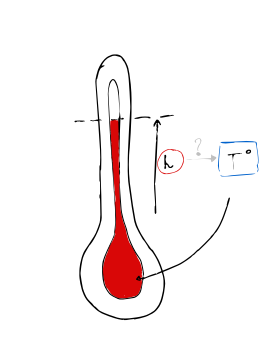
\includegraphics[clip, width=3cm]{Introduction/pics/therm_pb.png}
    \caption{Thermometer Graduation problem illustration. Given a simple liquid based thermometer, we aim at finding the matching between height of the liquid within the glass tube and temperature.}
    \label{fig:therm_calib}
\end{figure}

Let's consider a standard liquid based thermometer that consists of a liquid in a glass tube .
When interested in knowing the temperature, we observe the level of a thermometer.
In order to do so, someone had to graduate the thermometer. 
This seemingly simple action can be detailed in a two-step process, which involves the construction of a theoretical model and its calibration using real-world data.

The first step involves compiling theories and assumptions to construct a model linking the observed level and the actual temperature.
In this instance, based on our knowledge of fluid dilation in response to temperature, assuming the diameter of the tube is constant with height, we can posit that the level is linearly correlated with the temperature.
This model introduces two parameters: the slope and offset of our linear model that need to be ascertained.

The second step involves determining these parameters. This step requires some calibration data as inputs. They are traditionally obtained by immersing the thermometer in icing and boiling water to acquire the levels corresponding to 0°C and 100°C.
  Using those data points, a linear system can then be used to solve for the parameters. Which finally gives use our level-to-temperature mapping


The solution, therefore, is a product of both theory and data, and can be reduced to two key components: the model and the calibration algorithm.

Interestingly, the model's complexity can often be inversely proportional to the amount of data required. For instance, a model with fewer assumptions demands more data. If we were to abandon the assumption of the thermometer tube's constant diameter, we would need to incorporate a parameterization of the tube diameter in our model. This addition creates more parameters and consequently demands additional data for calibration.

Conversely, having access to more data can allow us to work with fewer assumptions. Suppose we possess a well-calibrated thermometer that can provide unlimited data points. In that case, we could reduce our assumptions to a minimum and rely heavily on empirical evidence, marking each thermometer graduation using data directly from our well-calibrated thermometer.

With these carefully calibrated graduations now etched onto our thermometer, we can use the liquid level as a convenient stand-in for the temperature. However, an important question remains: How can we verify the accuracy of our newly graduated thermometer?

\begin{figure}[h]
\centering
\begin{tabular}{ccc}

    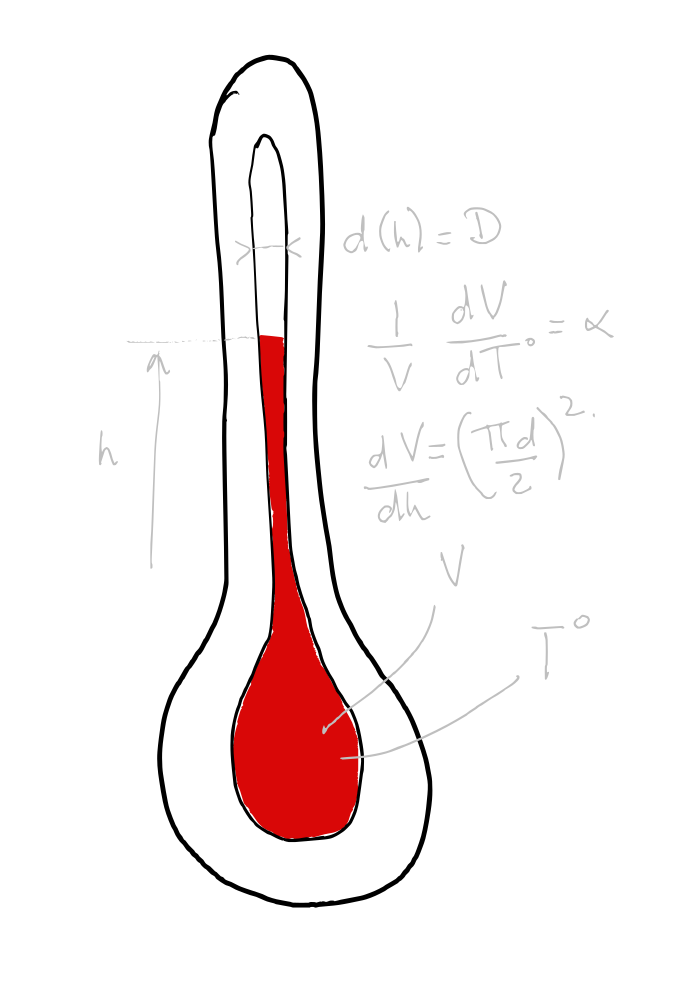
\includegraphics[clip, width=3cm, width=3cm]{Introduction/pics/therm_theroy.png} &   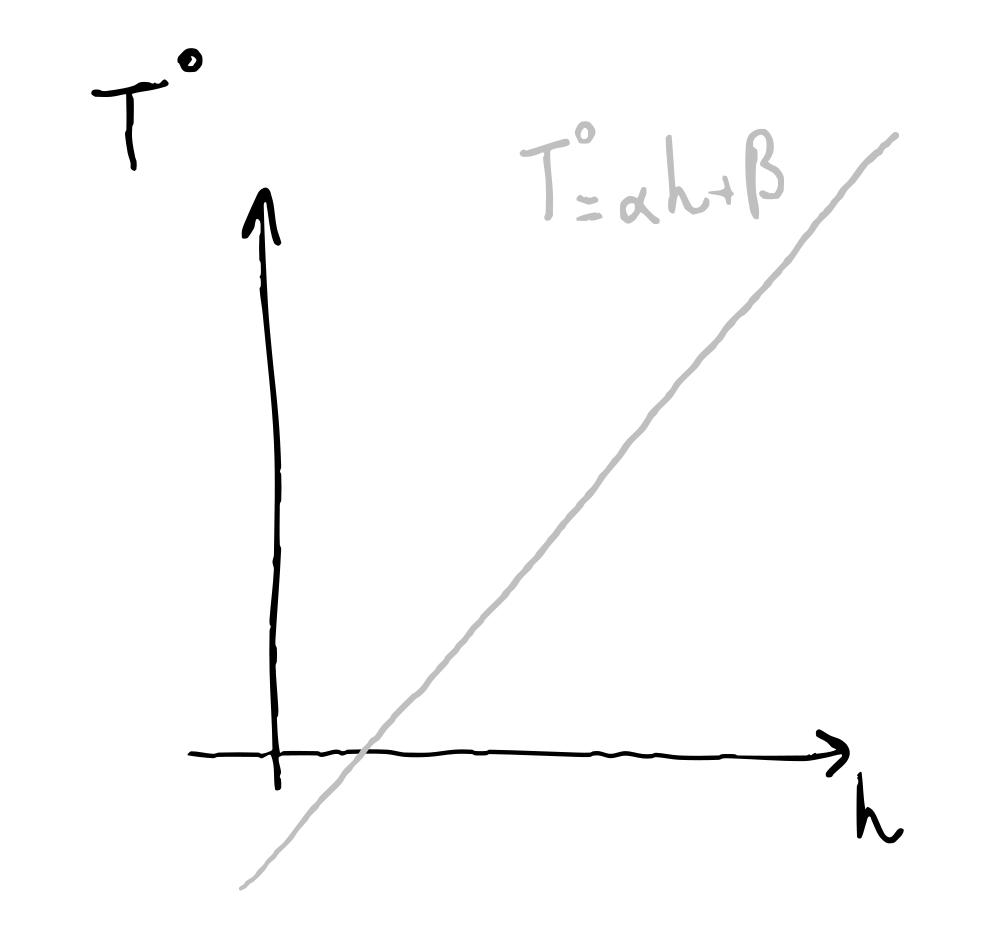
\includegraphics[clip, width=5cm]{Introduction/pics/therm_model.png}  &   \\   Assumptions & Model&\\ 
     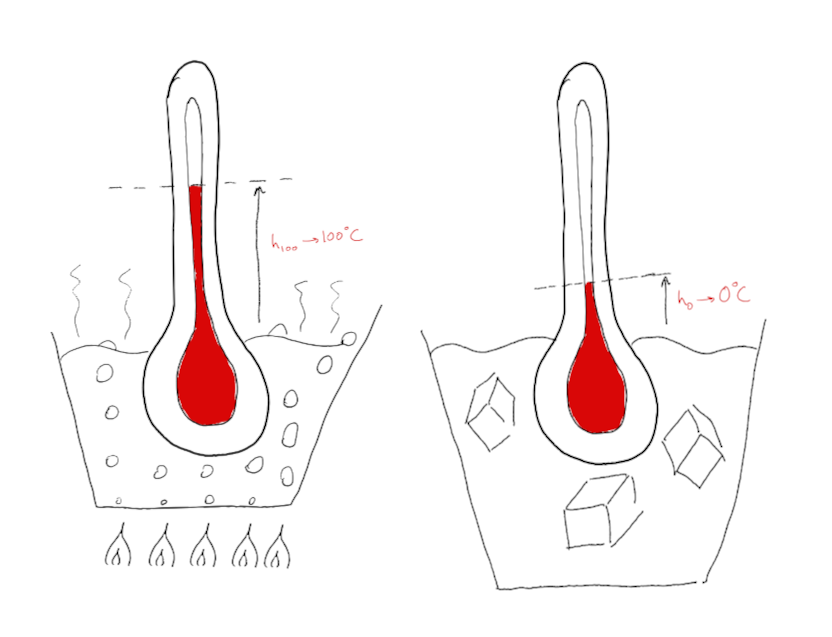
\includegraphics[clip, width=4cm, height=4cm, trim={2cm 1cm 2cm 2cm}]{Introduction/pics/therm_obs.png} &    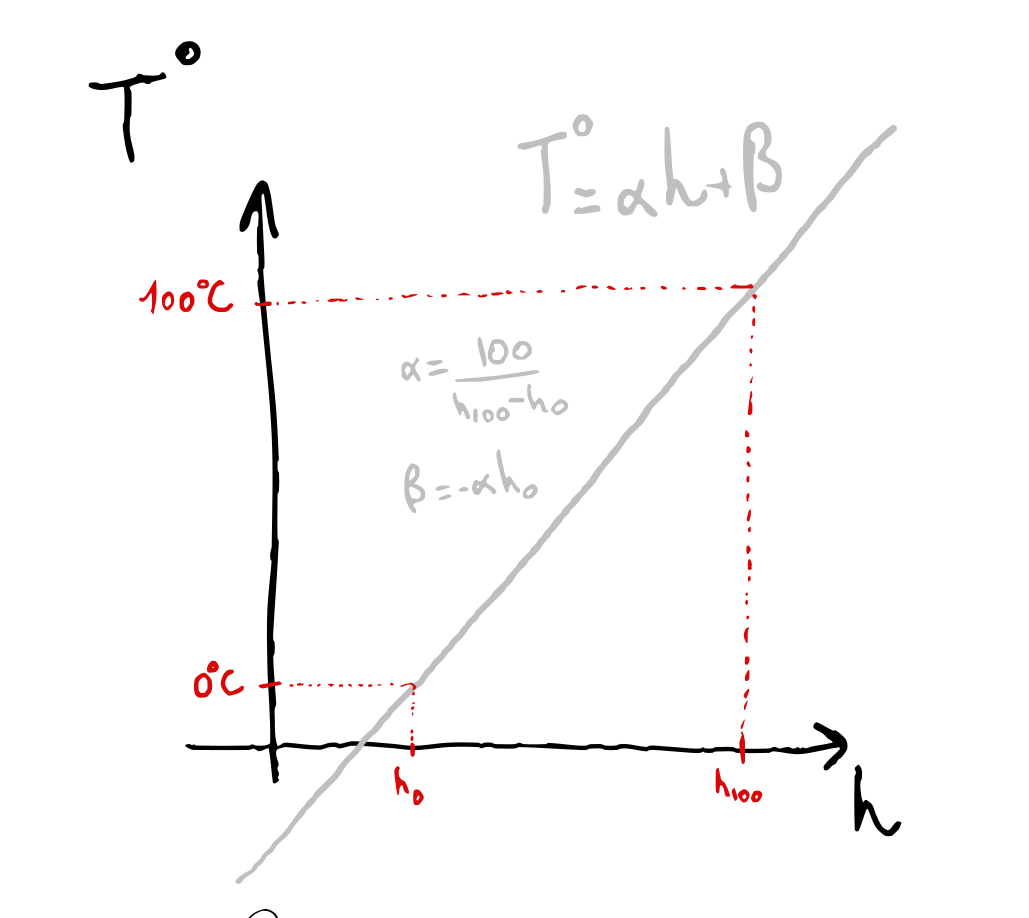
\includegraphics[clip, width=5cm]{Introduction/pics/therm_calib.png}   &  \\    Data & Calibration&\\
\end{tabular}

    \caption{Mapping thermometer level to temperature. The first step consists in compiling theoretical knowledge to determine a model of the level to temperature relationship. This model define the set of candidate graduations. The second step consists in leveraging data to chose the best candidate graduation through some calibration procedure.}
    \label{fig:therm_mapping}
\end{figure}

\subsection{Evaluation}

Without evaluation the use of our calibrated instrument would solely rely in the faith given to our mapping above.
However one may prefer quantifying the thermometers quality through metrics.

In our case the most intuitive metric for characterizing our thermometer's quality is be the precision of the graduations.
Note that is strongly dependent on the use of the instrument, some situations may put importance on other characteristic such at the range at which it's functional.
In order to properly evaluate our calibrated instrument, we need to test it in conditions corresponding to its intended use. (testing it domestic thermometer 5 kilometers underwater would not give a relevant evaluation).

 To do so, let's explicit some assumptions made on what we expect from our thermometer.
  For example that it needs to "be accurate to the half of degree", "have response time under 10 minutes", "work between -30°C and 200°C" "work at a reasonable atmospheric pressure" etc...

Then we need data to measure the precision of our thermometer in a way that is representative of how we want our thermometer to behave. Using a trustworthy reference like a third-party well-graduated thermometer, we could compare the measurements of the reference with the one given by our solution.
  An example evaluation procedure could be to confront the measurements of the two instruments at different temperatures such as: in a freezer, in a fridge, at ambient room temperature and in an oven.

Using the procedure above, we can compute our precision metrics and assess if the quality of our thermometer is acceptable.
This exercise, raises some critical points about evaluation. The process relies on two components that require a deep understanding of the thermometer's intended use: a suitable choice of metric and representative data. If the chosen metrics don't align with the intended use of the thermometer, the evaluation will be flawed. Similarly, if the data isn't representative of the thermometer's intended use, the evaluation will also be flawed.
 Furthermore, the reliability of the reference thermometer is pivotal. If the reference thermometer is not well-graduated, the best of metrics won't be able to correctly evaluate our thermometer. 

It's also crucial to differentiate between calibration data, which is used to determine the graduation, and evaluation data, which is used to assess the graduation's quality.
A well-functioning thermometer should provide accurate temperature readings even for levels it wasn't calibrated on. Thus, evaluation data should differ from calibration data. If we only measure precision at 0°C and 100°C, a thermometer that perfectly fits the calibration data would receive the highest metric, even if the other graduations were nonsensical.

\begin{figure}
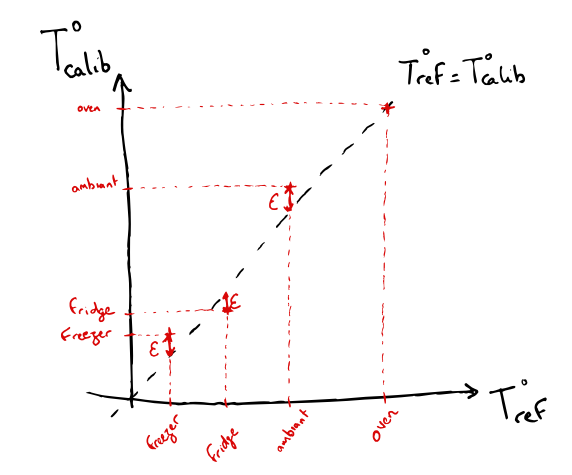
\includegraphics[clip, width=6cm]{Introduction/pics/errors.png}  
    \centering
    \caption{Evaluation and errors. Given some evaluation data and choice of metric, we can compute the errors associated with our graduation. $T^{\circ}_{calib}$ and $T^{\circ}_{ref}$ are respectively the temperatures given by our graduation and a reference well graduated thermometer}
    \label{fig:err_sources}
\end{figure}



 \subsection{Sources of errors}


\begin{figure}
\begin{tabular}{c|c|c}
     \hspace{-.15\linewidth}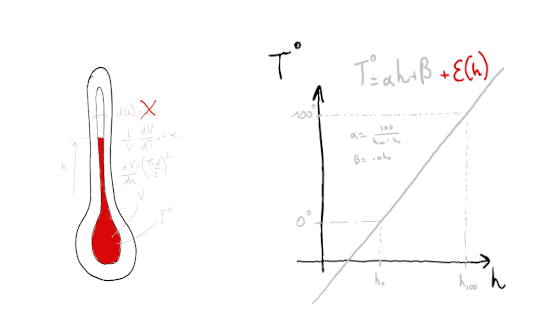
\includegraphics[width=.4\linewidth]{Introduction/pics/model_err_w_source.png}  &
     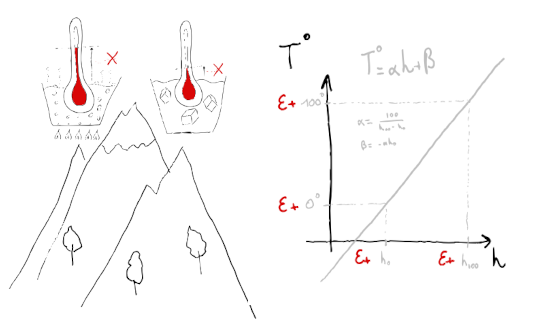
\includegraphics[width=.4\linewidth]{Introduction/pics/data_err_w_source.png} &
     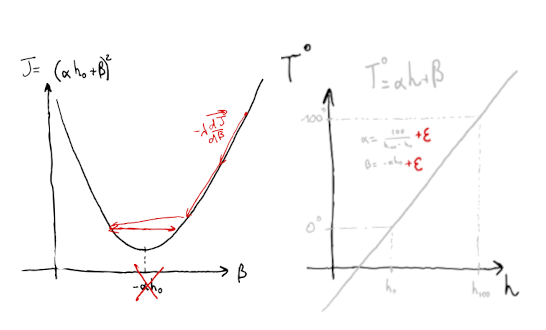
\includegraphics[width=.4\linewidth]{Introduction/pics/optim_err_w_source.png} \\
     \hspace{-.15\linewidth}Model &  Data &  Algorithm \\
\end{tabular}
    \centering
    \caption{Illustration of the different sources of errors for the thermometer graduation. From left to right: model errors result from erroneous assumptions about the system. Data errors result from inaccuracies in the calibration data and algorithmic errors result from a failure of the calibration procedure to select the best candidate from the model.}
    \label{fig:err_sources}
\end{figure}
Given an evaluation procedure, the errors are the gap to the reference and can be attributed to three sources: the model, the algorithm and the calibration algorithm.
 The model is a source of error if the assumptions made were inaccurate. For example if the diameter of the tube is not constant with height the linear relationship between level and temperature is not verified and will induce errors when interpreting the level.

 Even with perfect assumptions, noisy data can introduce errors in the calibration. If we interpreted our 0°C and 100°C in icing and boiling water at the top of a mountain with lower atmospheric pressure, we will have calibrated our parameters with erroneous measurements and the subsequent graduation of our thermometer will be inaccurate.

 Finally even with perfect assumptions and perfect data, the algorithm used to find the solution's parameters can be a source of errors if it fails to find the optimal parameters. For example if we solve for the parameters with a gradient descent method, using a step size too big will prevent finding the exact parameters which will also results errors in the subsequent measurements.

In order to develop a graduation procedure, we need to take those sources of error into account. The graduation procedure choice will not only depend on the level-temperature relationship but on the whole relationship between calibration data to the final calibrated thermometer. We therefore need to incorporate in our reasoning how the calibration data was acquired, what is the best model to map the level to the temperature, and what is the best algorithm to find the optimal parameters of the model.


This leads us to the following methodological problem "How to find the best thermometer graduation procedure?"

\subsection{Methodological framework}
In the process of finding a solution to the level-temperature mapping problem, we need to chose a model, an algorithm, and have access to calibration data. Additionally, to evaluate our solution, we need to define a metric and have access to evaluation data. Interestingly, these components can be specified at a higher level for solving and evaluating the graduation procedure itself, essentially creating a meta-level or "second order" problem.

The \textbf{Model}, in this second order scenario, combines different assumptions to determine the set of potential graduation procedures. 

The \textbf{Algorithm} is used to select the best graduation procedure. This could be as straightforward as testing different combinations and choosing the most effective one, or it could involve complex numerical optimization procedures to determine higher-level parameters.

The \textbf{Calibration Data}, at the second order, consists of graduation tasks with a method to assess the performance of candidate procedures. This allows the algorithm to select the best solution.

The \textbf{Evaluation Metric} should reflect the intended use of the graduation procedure, including the range of thermometers we plan to use this procedure for. A useful metric might be the precision of all the thermometers we aim to graduate using the proposed solution.

The \textbf{Evaluation Data} should be representative of the variety of intended uses. This means it should contain graduation tasks for a range of thermometers of interest. Additionally, we need a reference for these tasks to measure the precision of our solution.

By leveraging these five components, we can select the best calibration procedure, quantify its quality using the evaluation data, and use it to calibrate new thermometers with confidence in the resulting calibrated instrument. This parallels the problems of "Finding the level-temperature mapping" (which we refer to as the first order problem) and "Finding the graduation procedure" (the second order problem) and offers insights on where general purpose methodological tools can find applications.

Note that second order metrics can extend beyond the scope of the first order problem. These metrics could encompass aspects such as robustness to noise or the computational complexity of the calibration procedure. This means our evaluation of a calibration procedure not only includes how well it measures temperature, but also how well it handles uncertainties or computational burdens.

A second order solution can be conceptualized as a function. This function would accept first order calibration data as inputs, which contain observations of a specific thermometer and their corresponding temperatures. The output of this function would then be a first order solution - a tailored graduation for the thermometer represented in the data.

The second order problem also involves making decisions on parameters to select the best solution, which can take various forms. For instance, these parameters can be discrete choices between different assumptions, like whether to consider the thermometer's tube diameter as constant or not. The parameters can also denote choices between different first order algorithms like choosing a direct linear system inversion or a iterative optimization procedure. Lastly, these second order parameters can be constants in the level-temperature mappings or parameters of an optimization procedure, like step size. This shows that the parameters in the second order problem have a broad range of applicability, affecting both the details of the calibration procedure and how the procedure is chosen.

Finally, a critical note is that the data used to evaluate a solution at the second order level should still be separate from the calibration data. This principle holds true for the same reasons it applies to the first order problem - using distinct data sets helps to ensure that our solutions generalize well beyond the specific scenarios they were trained on.

\section{From toy example to ocean altimetry scenarii}
\subsection{Introducing space and time}
Our previous example implicitly solved the estimation problem of the liquid temperature  within the thermometer. However, we can extend the problem formulation to try to estimate the temperature in the room the thermometer is placed. This implies to take into account the duration required for the indicated level to reflect the accurate temperature of its location. This introduce a temporal consideration and therefore some dynamics about the system.

This dynamical scenario introduces a more complex case where the estimated temperature can depend from a series of observations over time. This shift has implications for the components of our method.

For instance, the evaluation metrics must now consider the dynamical characteristics of the thermometer calibration. The model must account for additional factors, including assumptions about how temperature diffuses over time. Similarly, the calibration algorithm and data used to select the best solution must adapt to these changes.

In this dynamical context, we have the choice of considering the dynamic aspect as a separate or joint problem to the calibration. We could treat the thermometer's level readings as direct observations or infer the dynamic temperature from the thermometer's liquid's temperature. These choices impact our assumptions about the model and the noise in the data.

Furthermore, we have until now focused on estimating a temperature value at a single location. However, this problem can be straightforwardly extended to the estimation of a temperature field across a spatio-temporal domain.

We can then formulate the more generic problem of temperature estimation from thermometer observations as follows:

\begin{itemize}
    \item First-order problem: Determine the temperature field in a room over a specific period, given observations from thermometer measurements at different places and times.
    \item Second-order problem: Determine a procedure that maps a set of observations to a temperature field.
\end{itemize}

\subsection{Notations}
Given the problem formulations above, the following notations can be introduced to encompass the first order problems of interest in this thesis.
Given some observations $y$ defined on a spatio-temporal domain $\Omega_y$ we want to estimate a quantity of interest $u$ on a domain $\Omega_u$. We are therefore looking for a mapping $f$ that estimate $u$ from $y$
The process of determining $f$ can be detailed in two steps, first determining the set $\cal{F}$ such that $f \in \cal{F}$ by making some assumptions on $f$. Then determining the calibration procedure $c$ that will use the calibration data $\cal{D}$ to select $f$ from $\cal{F}$
The evaluation of the solution rests on the choice of metrics $m$ and evaluation data $\cal{E}$

\subsection{Satellite altimetry}
The thermometer provided a good stepping stone to introduce the necessary concepts.
However the actual problem we're interested in is the estimation of the sea surface height (SSH) given satellite altimetry data.

In recent decades, Satellite NADIR altimeters have greatly improved our observational capabilities enabled by providing a global coverage 

However due to the scarce and irregular sampling of altimeter constellations, current operational products do not yet resolve processes with horizontal scales smaller than 150 km\cite{}.
These processes linked to the mesoscale and submesoscale dynamics of the ocean surface play an important role in the heat redistribution within the ocean, which has implications for climate monitoring.
The recent deployment of the novel KaRIN sensor during the SWOT satellite mission\cite{} provides opportunities to address this gap.
This new sensor will provide unprecedented two dimensional images of the ocean surface topography but will also introduces calibration challenges\cite{} due to previously unseen errors.
Additionally these new data are expected to enhance the reconstruction of SSH maps.

The process of graduating a thermometer, as previously illustrated, shares fundamental methodological parallels with the task of estimating sea surface height (SSH) using satellite data.
Just as we use a thermometer to measure temperature by observing the liquid level, satellite altimetry allows us to estimate the SSH by interpreting specific signals and measurements from a much larger and more complex system.

In both cases, we observe certain behaviors — be it the level of liquid in a thermometer or the satellite observations of the ocean surface — and use these to infer something about the underlying state of the system we are interested in. Both rely on the creation of a model based on existing knowledge and assumptions, and tuning that model using calibration data to map observed behavior to the desired quantity.

The temporal aspect is also shared. Much like the response time of a thermometer, which determines how quickly it can accurately measure the temperature of its environment, satellite data gives us a series of snapshots over time from which we can reconstruct the dynamic behavior of the sea surface.

When considering the spatial dimension, satellite altimetry provides sparse measurement of the ocean surface and estimating SSH is like placing thermometers across a room to understand the distribution of temperature in that space. The same principle is applied to satellite altimetry, but on a much larger scale, mapping the Earth's oceans.

In essence, both cases involve observing a system, interpreting those observations through a theoretical model, and refining that model with real-world data to obtain the most accurate estimation possible. The application and scale are vastly different, but the underlying principles of observation, modeling, calibration, and evaluation are consistent.

This manuscript, therefore, aims to explore the application of deep learning to two key observation problems related to these issues. The first is estimating SSH from noisy SWOT observations, and the second is inferring the complete SSH field from partial measurements which we detail in the following two sections.
  
\subsection{SWOT Calibration}

  \begin{figure}
      \centering
            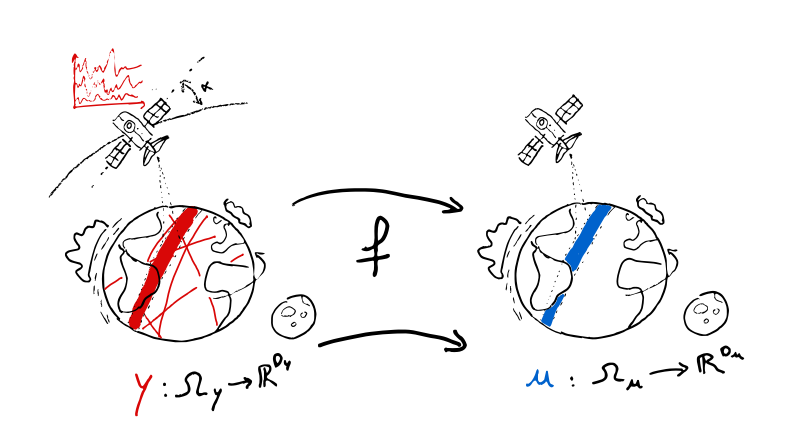
\includegraphics[width=\linewidth]{Introduction/pics/calib_task.png}    
      \caption{SWOT calibration. The left part illustrate the observed domain in red while the right part indicates the domain on which we aim at estimating the SSH.}
      \label{fig:calibration_task}
  \end{figure}
The first observation problem we address is the estimation of sea surface height on the domain observed by the KaRIN instrument of the SWOT mission from scarce calibrated altimetry observations and uncalibrated SWOT observations.
As mentioned above, the KaRIN instrument deployed during the SWOT will contain both unprecedented errors and information about the sea surface height.
We are more precisely interested in the removal of correlated errors due to systematic instrument errors and noise-inducing geophysical processes.



\subsection{Altimetry Mapping}

  \begin{figure}
      \centering
            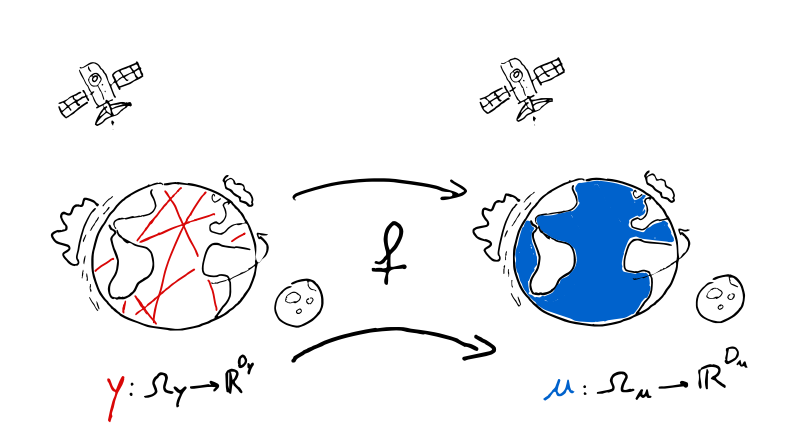
\includegraphics[width=\linewidth]{Introduction/pics/mapping_task.png}
      \caption{Nadir Altimetry mapping. The left part illustrate the observed domain in red while the right part indicates the domain on which we aim at estimating the SSH.}
      \label{fig:mapping_task}
  \end{figure}

The second observation problem we address is the estimation of sea surface height on daily maps from scarce calibrated altimetry observations.
This can be viewed as an spatial and temporal interpolation of sparsely observed SSH to a dense domain.
Contrary to the KaRIN calibration which is a novel task, the mapping of NADIR altimeter task has been addressed by a variety of methods.
Those methods use different assumptions and algorithm to estimate the maps of SSH.


\section{Deep learning: opportunities and challenges}

\subsection{Success stories in computer vision and natural language processing}
Deep learning brings forth models, such as neural networks, that are predicated on very weak assumptions. Their strength lies in the fact that, given sufficient parameters, they can approximate any function\cite{}. This leads to deep learning models defining vast sets of potential candidates, consequently requiring substantial datasets and sophisticated algorithms to find the best fit.

Innovations in model architectures such as ResNet\cite{}, batch normalization\cite{}, and in optimization procedures\cite{} like Stochastic Gradient Descent (SGD)\cite{}, Adam\cite{}, and various learning rate schedules have consistently improved the search of larger spaces for candidate solutions, therefore enabling the use of larger neural networks. 
However, the fact that deep learning models can in theory approximate any function introduces a peculiar consideration which is that fitting exactly the calibration data gives you no guarantee on how the model will behave on unseen data.
The gap of performance between "seen" and "unseen" data is called the generalization gap.
This has standardized the practice of splitting the calibration data in two sets: training and validation.
The training set is used by the optimization procedure to search for the parameters whereas the validation set is used to assess the quality of each candidate. 
Addressing the problem of generalization have motivated many innovations in regularization, architectures, initialization schemes and data augmentation techniques.


When looking at different application domain, the track records of deep learning in computer vision\cite{} and natural language processing\cite{} are especially impressive. 
The combination of models and algorithm brought by deep learning have managed to solve tasks that were previously unsolved.
Indeed the universality of deep learning models have brought a big leap forward in tasks such as generic image recognition or next word prediction which are very hard to model using theoretical knowledge.

Presented as such deep learning seems to provide universal tools,  
however we would like to stress two factors that seem of great importance when looking at the contributions of deep learning in specific fields.
The first factor is quality and availability of data.
Indeed the creation of large, curated datasets, like ImageNet\cite{} in computer vision or ThePile\cite{} in natural language processing have shown to dramatically expedite the development of novel approaches. 
The second factor is the design of informed architectural patterns that are particularly suited to the domain, leading to performance breakthroughs.
Examples of these include convolution techniques\cite{} and U-Net architectures\cite{} in computer vision, and attention mechanisms\cite{} in natural language processing.


\subsection{Deep learning for ocean altimetry}
Given a observation problem stated as above, deep learning brings to the table its set of tools for defining candidate solutions to a problem as well as optimization procedures for searching this set for the optimal candidate.
Notice that these tools are generic enough to be used for both order of problems. For example when applied to altimetry mapping, deep learning architectures can used to directly model the SSH field with neural fields\cite{}. In this case the model is calibrated on a single set of observations.
They can also be used to model the mapping procedure itself\cite{} and in this case the model will be calibrated on multiple sets of observations.

When comparing altimetry to previously mentioned deep learning application domain, we note some specificities.
On one hand extensive theoretical knowledge has been accumulated on the physical processes that give structure to the data and that explicitly links the observations with the quantities of interests.
This raises the question on the advantages of generic purpose models when domain expertise can inform tailored ones explicitly accounting for the system dynamics.
And domain experts have successfully exploited that to solve different observation problems.

On the other hand the available data made of instrument measurements, observation products, and numerical model outputs, although consequent, introduce challenges by the lack of the ground truth quantity we want to estimate. (The best we can do is consider a calibrated instrument as ground truth when available). This is the case for both the altimetry use-cases considered.
Note that the lack of ground-truthed dataset introduce challenges both for the calibration of the model as well as for the evaluation of the method.


This manuscript will specifically look at how domain knowledge and available data can be used to benefit from the deep learning advances for altimetry analysis.



\section{Thesis objectives and outline}

The following chapters of this thesis are organized as follows:

\textbf{Chapter 2} addresses the relevance of deep learning architectures for the calibration of correlated errors in SWOT data.
From an applicative standpoint, the flexibility of deep learning methodology opens the potential for capturing signals that are tricky to explicitly parameterize.
From a methodological perspective, this study shows how deep learning architectures can be tailored with assumptions on the instrument and its measurements.
More specifically, this is done by using the spectral specifities of the errors can be leveraged to design a efficient neural calibration scheme.
This study bypasses the challenges brought by the lack of ground-truthed dataset.
It takes place in a simulated setup with the SSH and error signals are simulated and therefore known.


\textbf{Chapter 3} tackles more specifically the data availability problem. It studies how neural mapping schemes can be applied to real data.
It looks more specifically at the 4DVarNet\cite{} framework which has been demonstrated in a simulated setup\cite{} using simulated SSH for training and evaluation.
This chapter look at the performance of deep learning models trained on simulated data.
It shows how the extensive physical knowledge of the ocean dynamics can be leveraged to palliate the lack of ground-truthed dataset in altimetry through the use  of numerical simulations for training.

\textbf{Chapter 4} considers the more practical scientific question of how to maximize the synergies between the ocean altimetry and deep learning community.
Both fields are well established with accumulated knowledge, conventions, and best practices. 
As described in this chapter, deep learning brings powerful models and algorithms.
However the evaluation data and metrics of an altimetry product can only be sensibly designed by an domain expert. 
We propose OceanBench, an interface in the form of a software suite of tools.
Oceanbench aims at empowering domain experts to easily design altimetry problems of interests and qualifying them with relevant metrics. 
It then provides machine learning practitioners access to the necessary data as well as suited utilities for 

\textbf{Chapter 5} discusses and concludes on the research presented in this manuscript. We summarize the main objectives and results in previous chapters as well as proposing some future avenues of research.
 
\end{bibunit}

